% !TeX encoding = UTF-8
% !TEX root = ./presentation.tex
\section{\Design\ de Sistemas Embutidos}

   \begin{frame}
      \begin{itemize}
         \item Metodologia baseada em \parencite{Sass2010, Arato2003, Arato2005, Mann2007, Hassine2017}.
      \end{itemize}
   \end{frame}

   \subsection{\Design\ Referencial de \Software\ Utilizando Grafo de Controle de Fluxo}

   \begin{frame}{Grafo de Controle de Fluxo (GCF)} \vspace{-1em}
      \begin{itemize}
         \setlength{\itemsep}{1.2em}
         \item Descrever um sistema, tanto em \software\ ou \hardware, livre de uma especificação de forma
         \begin{itemize}
            \item Desenvolvendo rápidos protótipos, referenciado como \design\ de referência de \software.
         \end{itemize}

         \item Generalização de uma especificação bastante completa, eliminando qualquer tipo de incertezas sobre o comportamento do sistema com o simples fato de analisar o \design\ referencial do \software.

         \item O sistema inicial é dado como grafo de tarefas/rotinas, define-se \bx{$ C = (B, F) $} onde $B$ são vértices que representam os blocos básicos e $F$ são arestas que indicam a todas as possibilidades de caminhos entre os blocos.

      \end{itemize}
   \end{frame}

   \begin{frame} %\vspace{-1em}
      \begin{figure}[h] \centering
         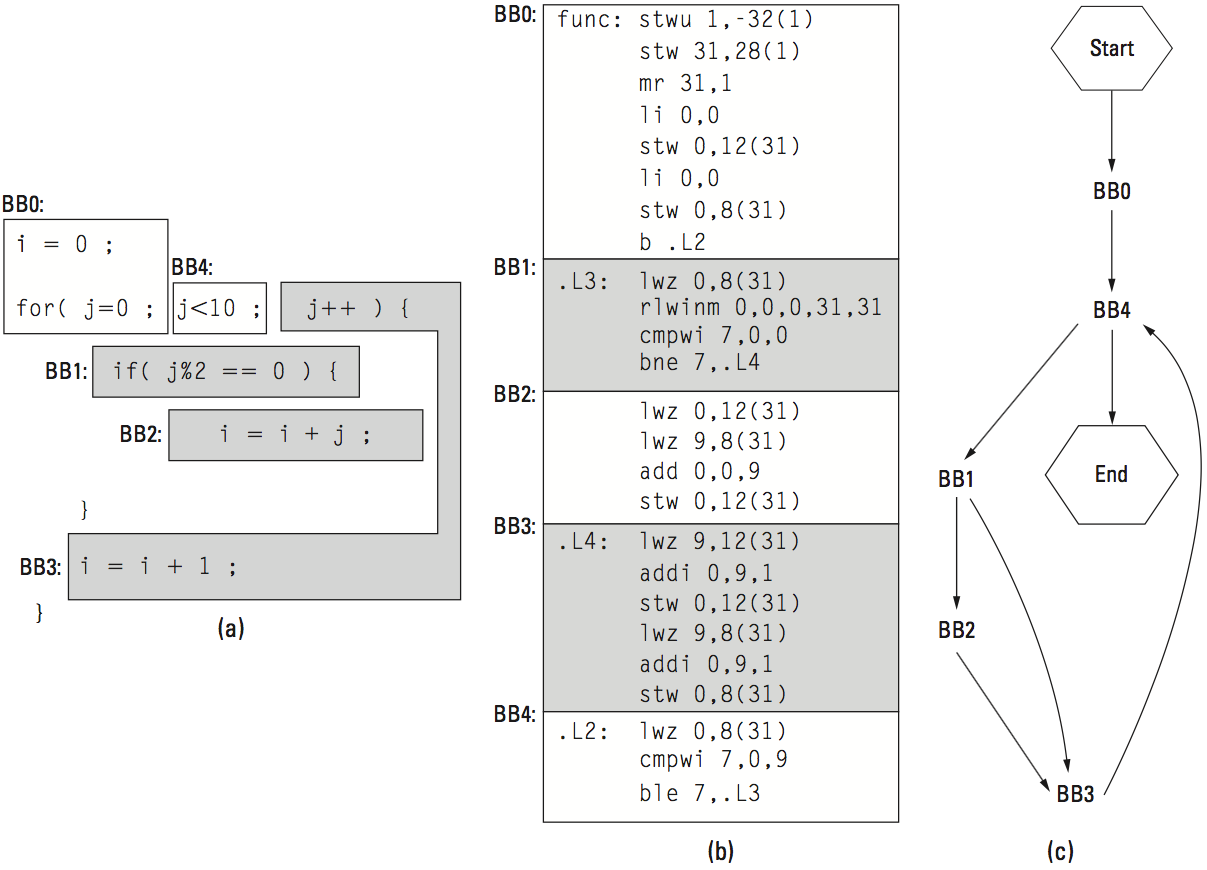
\includegraphics[width=0.89\textwidth]{img/f3-6.png}
         \caption{Identificação de blocos básicos e a representação de cada modelo de descrição de \software.}
         %\label{fig:f3-6}
      \end{figure}
   \end{frame}

   \begin{frame}{Grafo de Controle de Fluxo (GCF)}
      \begin{itemize}
         \setlength{\itemsep}{1.6em}
         \item A decomposição de um DRS pode gerar dois componentes:
         \begin{itemize}
            \item Porção a ser realizada em \hardware\ e outra executada em \software;
         \end{itemize}

         \item Essa decisão de divisão é chamada de problema de particionamento.

         \item Para sistemas baseados em Plataformas FPGA, particionamento é um sub-problema de um problema mais geral localizado no \codesign, onde refere-se ao \design\ cooperativo.
      \end{itemize}
   \end{frame}


   \subsubsection{Grafo de Chamada (GC)}

   \begin{frame}{Grafo de Chamada (GC)}
      Modelado uma sub-rotina de um DRS utilizando o GCF, define-se o Grafo de Chamada (GC).

      \begin{itemize}
         \setlength{\itemsep}{0.6em}
         \item Consiste num conjunto de GCFs, um por sub-rotinas, ou seja, \bx{$\mathcal{C} = {C_0, C_1, \dots C_{n-1}}$}
         %onde $ C_i = (V_i, E_i) $
         onde $ C_i = (B_i, F_i) $ representa o GCF de uma sub-rotina $ i $.

         \item Sendo assim, o grafo estático de chamada da aplicação é escrito por \bx{$\mathcal{A} = (\mathcal{C}, \mathcal{L}) \label{eq:a}$} onde
         \begin{itemize}
            \item \A\ representa uma aplicação específica e;
            \item $ \mathcal{L} \subseteq \mathcal{C} \times \mathcal{C} $.
         \end{itemize}

      \end{itemize}

      \begin{block}{Duas sub-rotinas são relacionadas}
         Se podem ser determinadas, no tempo de compilação, que a sub-rotina $ i $ tem potencial de invocar a sub-rotina $ j $, ou seja, \bx{$ (C_i, C_j) \in \mathcal{L} $}.
      \end{block}
      \pdfnote{Para entendimento da partição}
      \pdfnote{um subconjunto do plano cartesiano dos GCF}
   \end{frame}


   \begin{frame}{Definição de Partição}

      Uma partição $ \mathcal{S} = \{S_0, S_1, \dots\} $ de um conjunto universal $ U $ é um conjunto de subconjuntos de $ U $ sendo que
         %
         \begin{equation}
            \bigcup_{S \in \mathcal{S}} S = U \label{eq:part_form_1}
         \end{equation}
         \begin{equation}
            \forall S, S' \in \mathcal{S} | S \cap S' = \emptyset \label{eq:part_form_2}
         \end{equation}
         e assim
         \begin{equation}
            \forall S \in \mathcal{S} \cdot S \neq \emptyset \label{eq:part_form_3}
         \end{equation}
         %

            \bigskip

         \begin{description}
         \setlength{\itemsep}{0.6em}
            \item [Equ. \ref{eq:part_form_1}:] cada elemento de $ U $ é um membro de, pelo menos, um subconjunto $ S \in \mathcal{S} $;

            \item [Equ. \ref{eq:part_form_2} e \ref{eq:part_form_3}:] os subconjuntos $ S \in \mathcal{S} $ são emparelhados disjuntos e não vazio.

         \end{description}

      \pdfnote{Em outras palavras, cada elemento do nosso universo $ U $ termina exatamente em um dos subconjuntos de $\mathcal{S}$ e nenhum dos subconjuntos são vazios.}
   \end{frame}


   \begin{frame}{Definição de Partição}

      Uma partição $ \mathcal{S} = \{S_0, S_1, \dots\} $ de um conjunto universal $ U $ é um conjunto de subconjuntos de $ U $ sendo que
         %
         \begin{equation}
            \bigcup_{S \in \mathcal{S}} S = U \label{eq:part_form_1}
         \end{equation}
         \begin{equation}
            \forall S, S' \in \mathcal{S} | S \cap S' = \emptyset \label{eq:part_form_2}
         \end{equation}
         e assim
         \begin{equation}
            \forall S \in \mathcal{S} \cdot S \neq \emptyset \label{eq:part_form_3}
         \end{equation}
         %

            \bigskip

         \begin{itemize}
            \item Considere $ U = \{a, e, i, o, u, y\} $. Uma partição $ \mathcal{X}_i $ de $ U $:

         \end{itemize}
         \begin{eqnarray}
         \mathcal{X}_a &=& \left\{\{a, e, i, o, u\}, \{y\}\right\} \label{eq:xa} \\
         \mathcal{X}_b &=& \left\{\{a\}, \{e\}, \{i\}, \{o\}, \{u\}, \{y\}\right\} \label{eq:part_a} \\
         \mathcal{X}_c &=& \left\{\{a\}, \{e\}, \{i\}, \{o\} \right\} \label{eq:part_c} \\
         \mathcal{X}_d &=& \left\{\{a, e, i\}, \{i, o, u, y\}, \{\}\right\} \label{eq:part_d}
         \end{eqnarray}
       \pdfnote{c viola a 1 (omite y) e a d viola 2 e 3 (conjunto vazio além de redundância). }
   \end{frame}


   \begin{frame}{Aplicar o formalismo à $\mathcal{A} = (\mathcal{C}, \mathcal{L})$}
      \begin{itemize}
         \item Se assumirmos o universo é o conjunto de todos os \textit{blocos básicos} $B$ de todas as sub-rotinas de um dispositivo \wearable, então $U$ é as partições de sub-rotinas
         %
         \begin{equation}
            U = \bigcup_{C \in \mathcal{C}} B(C) \label{eq:bigcup}
         \end{equation}
         ou seja,
         \begin{equation}
            \mathcal{S}  = \left \{
            \underbrace{\left \{ b_0, b_1, \dots, b_i \right \}}_{\text{sub-rotina }C_0},
            \underbrace{\left \{ b_i, b_{i+1}, \dots, \right \}}_{\text{sub-rotina }C_1},\dots
            \underbrace{\left \{ b_j, b_{j+1}, \dots, \right \}}_{\text{sub-rotina }C_{n-1}}
            \right \}
         \end{equation}

         \item Propósito
         \begin{enumerate}
            \item Reorganizar a partição de blocos básicos e então;
            \item Mapear cada subconjunto de ambos os \hs.
         \end{enumerate}

      \end{itemize}
   \end{frame}


   \begin{frame}{Aplicar o formalismo à $\mathcal{A} = (\mathcal{C}, \mathcal{L})$}
      \begin{itemize}

         \item Dessa forma pode-se
            \begin{itemize}
               \item Criar e remover subconjuntos não vazios;
               \item Mover blocos básicos ao redor até ter uma nova partição.
            \end{itemize}

         \item Obtém um novo resultado $ \mathcal{A}’ = (\mathcal{C}’, \mathcal{L}’) $, inferido a partir da reorganização da partição $ \mathcal{X}’ $.

            \bigskip

         \item Em seguida, basta mapear cada subconjunto de $ \mathcal{X} $ para ambos \hs

      \end{itemize}
         { \footnotesize
         \begin{equation}
            \mathcal{X}'   = \left \{
            \underbrace{
               \underbrace{
                  \left \{ b_j, b_{j+1}, \dots, \right \}
               }_{\text{sub-rotina }C_k}
               \underbrace{
                  \left \{ b_k, b_{k+1}, \dots, \right \}
               }_{\text{sub-rotina }C_l}
               \dots
            }_{\text{\software}}
            \
            \underbrace{
               \underbrace{
                  \left \{ b_0, b_1, \dots, b_i \right \}
               }_{\text{sub-rotina }C_r}
               \underbrace{
                  \left \{ b_i, b_{i+1}, \dots, \right \}
               }_{\text{sub-rotina }C_s}
               \dots
            }_{\text{\hardware}}
            \right \} \label{eq:part_final}
         \end{equation}
         }
   \end{frame}


   \subsection{Ganho de Performance}

   \begin{frame}
      \begin{itemize}
         \item Mundo \software\ possui análise de ordem de complexidade, em \hardware\ não possui-se um guia geral para comparação.

         \item Dessa forma, analisa-se por meio do ganho de performance
         \begin{itemize}
            \item ``Acumulação de pequenos ganhos que deveriam ser perdido numa aplicação direta na teoria de complexidade.''
            \item \Software\ utiliza-se de \profile, meta mais próxima para aferição em \hardware.
         \end{itemize}

         \item $ s(i) $ representa o tempo de execução esperado para uma invocação de uma sub-rotina $ i $, ou seja, bloco básico.
      \end{itemize}
   \end{frame}


   \begin{frame}
      \begin{itemize}
         \item Par o \hardware, assume-se que $ h(i) $ é o tempo de execução em \hardware.

         \item A `interfaceação' entre \hs\ requer tempo. Pode-se aproximar deste custo pela
         \begin{itemize}
            \item Aproximação do montante gasto na transferência de um estado ou o custo de configuração e latência.
            \item São representados por $ m(i) $ para recursos $ i \in \mathcal{H} $, sendo $\mathcal{H}$ o conjunto de recursos do \hardware.
         \end{itemize}

         \item $ \gamma $ representa o ganho de performance, ou seja, \speedup.

         \item Assim, qualquer subconjunto de blocos básicos que \textit{não produz um ganho de performance}, pode ser excluído.
         \begin{itemize}
            \item Ou seja, somente subconjuntos de blocos básicos para qual $ \gamma > 1.0 $ são considerados recursos candidatos.
         \end{itemize}

      \end{itemize}
      \pdfnote{y = gamma}
   \end{frame}

   \begin{frame}{\Speedup}

      \begin{equation}
         \gamma =
         \frac{
            \text{\textit{hardware speed}}
         }{
            \text{\textit{software speed}}
         }
         =
         \frac{
            \frac{
               1
            } {
               \text{\textit{hardware time}}
            }
         } {
            \frac{
               1
            }{
               \text{\textit{software time}}
            }
         }
         =
         \frac{
            \text{\textit{software time}}
         } {
            \text{\textit{hardware time}}
         }
      \end{equation}

      \begin{itemize}
         \item Performance individual de cada recurso $ \gamma(i), i \in \mathcal{C} $
      \end{itemize}
   
     \begin{equation}
        \gamma(i) = \frac{s(i)}{h(i) + m(i)}
     \end{equation}
      
      onde:

  
      \begin{description}
          \item [$ h(i) $ e $ s(i) $:] tempo de execução de uma implementação de um recurso $ i $ em \hs; e 
          
          \item [$ m(i) $:] é o tempo que se leva para sincronização, ou seja, o tempo que leva para guiar um dado entre o processador e o item reconfigurável.
      \end{description}
      \pdfnote{y = gamma}
   \end{frame}

   \begin{frame}
      \begin{block}{A Velocidade da Aplicação}
         É dependente dos \textbf{ganhos de performance do recurso} e o \textbf{quão frequentemente ele é utilizado} no \design\ referencial de \software.
      \end{block}
   
      \begin{itemize}
         \item Pode-se ter essa fração do tempo de um recurso particular $ p(i) $ a partir de informações de \textit{profile}.
         
         \item Dessa, usando $\gamma(i) = \frac{s(i)}{h(i) + m(i)}$, forma-se o \speedup\ da aplicação no geral:
      \end{itemize}
   
      \begin{equation}
         \Gamma = \left [
         (1 - p(i))
         +
         \frac{
            p(i)
         }{
            \gamma(i)
         } \right ]^{-1}
      \end{equation}
      
      \begin{description}
         \item [$\gamma(i)$:] performance individual de cada recurso (acelerador);
         \item [$p(i)$:] fração de tempo de um recurso particular (\software).
      \end{description}
      
      \pdfnote{A inversão estamos movendo entre taxa de execução e tempo de execução, mantendo o sentido de GanPerf.}
      \pdfnote{aumentando a velocidade do h de um 1 recurso tem menos e menos impacto na performance da aplicação a medida que sua frequência DECRESCE.}
   
   \end{frame}

   \begin{frame}
      \begin{itemize}
         \item Para aumentar a performance sistêmica no geral, aumentar-se a performance de componentes individualmente.
         
         \item \Speedup\ de múltiplos recursos em \hardware\ $ \mathbb{D} $
         
         \begin{equation}
            \Gamma (\mathbb{D}) =
            \left [
            1 + \sum _{i \in \mathbb{D}} \left (
            \frac{
               p(i)
            }{
               \gamma(i)
            }-p(i)
            \right)
            \right ]^{-1} \label{eq:d_final}
         \end{equation}
         
      \end{itemize}
      \pdfnote{Cada membro contribui à performance do sistema.}
   \end{frame}
   
   \begin{frame}{Consideração de Recursos}
      \begin{itemize}
         \item Uma tentativa seria a adição de recursos na abordagem $\sum_i p_i$.
         
         \item FPGA possui número finito de recursos disponíveis.
         
         \item Um meio de aproximação de recursos é \textbf{contar o número de células lógicas requeridas para cada recurso}.
         \begin{description}
            \item [$ r_{FPGA} $:] representará o total de números de células lógicas disponíveis.
            
            \item [$ r(i) $:] quantidade de células lógicas por cada recurso $ i $.
            
         \end{description}
         
         $$$ \sum_{i \in \mathbb{D}} r(i) < r_{FPGA} $$$
         
         %
         \begin{equation}
         \vec{r}_{FPGA} =
         \begin{pmatrix}
         r_{Logic\ Cells} \\
         r_{Memory}\\
         r_{DSP}\\
         \vdots \\
         r_{n-1}
         \end{pmatrix}
         \end{equation}
         %
         e com isso,
         %
         \begin{equation}
         \sum_{i \in \mathbb{D}} \vec{r}(i) < \vec{r}_{FPGA}
         \end{equation}
         %
         onde $ \mathbb{D} $ é o conjunto de recurso incluídos no \design.
         
      \end{itemize}
      \pdfnote{Implementar tudo em h ignorando custos de desenvolvimento/recursos.}
   \end{frame}

\begin{comment}

      


         %Infelizmente\todo{a}, esse modelo não leva em consideração o fato de que alguns recursos alocados podem interferir em outros, além de que a estimativa de performance é frequentemente baseada na suposição que recursos são próximos um do outro e recursos de rotas não são parte integral do modelo.


%\chapter{O Particionamento de \HS\ para Sistemas \Wearable} \label{chap:desenvolvimento}
   \section{O Particionamento de \HS\ para Sistemas \Wearable} \label{sec:desenvolvimento}

      De início, será considerado como aplicação \wearable\ um conjunto de instruções organizadas, e como visto na Seção \ref{sec:gc}, esta também representada por uma coleção de grafos de controle de fluxo, ou seja, grafo de chamada, especificando a sua ordem de execução.
      A partir deste, será feito análises a fim da procura de um particionamento que atenda aos requisitos de dispositivos \wearables, como alto poder de processamento sem o \textit{trade-off} de energia, além de miniaturização, confiabilidade e outros.

      Após esclarecidos algumas definições prévias (Seção~\ref{sec:definicoes_previas}), será apresentado o problema na Seção~\ref{sec:declaracao_problema}.
      %Alguns fatores podem ajudar nas decisões de particionamento tal como expectativa de ganho de performance (Seção \ref{sec:ganho_performance}) e os recursos utilizados em \hardware\ (Seção \ref{sec:recursos}).%, a forma na qual são usados e, talvez os mais importantes, quanto de sobrecarga de comunicação a decomposição impõe (Seção \ref{sec:comunicacao}) \todo{deixar?}e dificuldade de implementar um conjunto específico em \hardware\ (Seção \ref{sec:dificuldades}).\todo{organizar}

      \subsection{Definições Prévias} \label{sec:definicoes_previas}
         \begin{description}
            \item [Recurso:] grupo conectado de instruções de uma aplicação de \design\ referencial de \software\ `adequado' para uma implementação em \hardware.

            O recurso pode variar de um pequeno conjunto de instruções até um modulo de \software\ completo consistente de múltiplas sub-rotinas.
            Como o tamanho dos recursos afetam na performance, a decisão de implementação em \hardware\ depende da sua melhoria no sistema por inteiro e mensura-se os recursos utilizados com relação a outros recursos candidatos.

            Se determinado que o recurso é vantajoso, então os recursos de implementação em \hardware\ aumentam a arquitetura de \hardware;

            \item [Implementação em \hardware:] recurso adicional de uma específica aplicação;

            \item [Adequado:] descrevendo de forma mais geral no âmbito de sistemas \wearable, é a definição da situação na qual o projetista do sistema antecipa a percepção de vantagens na implementação em \hardware.
            %Para obter uma boa partição, geralmente deve-se examinar grupos que podem ser maiores ou menores que sub-rotinas definidas pelo programador.
         \end{description}

         %\section{Declaração Formal do Problema}
         %	Descreveremos problema segundo a definição de \citeauthor{Arato2005, Mann2007} a seguir.

         %\section{Solução analítica para particionamento}
         %\section{Visão Analítica Para o Particionamento}


      \subsection{Declaração do Problema} \label{sec:declaracao_problema}
         Nesta seção serão apresentadas as declarações matemáticas do problema de agrupamento de instruções em recursos e seus mapeamentos em \hardware\ ou \software, ou seja, o particionamento \hs.
         %Segundo \cite{Sass2010}, a forma mais comum de transcrever é descrever manualmente o \core\ com um HDL utilizando \design\ referencial de \software\ como especificação, método utilizado para descrever o problema.

         No particionamento, muitos problemas práticos impactam diretamente na performance do sistema.
         Nem todos os problemas podem ser incorporados num modelo analítico \cite{Wang2016}, e por isso, só podemos esperar que as soluções matemáticas produzam uma uma resposta aproximada ao problema de particionamento ao utilizar a declaração formal.

         Muitas das entradas do modelo são estimadas ou aproximações no qual futuramente degrada a fidelidade de resultados.
         %%Este é um fato relevante pois com isso, resolvendo o problema de particionamento `no papel', tem-se um particionamento que é próximo ao ótimo.
         %%Assim, cabe ao \designer\ ser habilidoso em usar os guias e projetar uma solução mais refinada.
         Dessa forma, é mais eficiente usar uma combinação de técnicas \textit{ad hoc} e matemáticas para encontrar uma solução ótima ou aproximada do que simplesmente confiar numa intuição.


         %\begin{comment}
         %\section{Declaração do Problema}
         Já descrito as ferramentas matemáticas necessárias para descrever o problema fundamental do particionamento no Capítulo \ref{chap:revisao_bibliografica}, pode-se então descrever formalmente o problema em termos de variáveis. % e descrever um algoritmo \todo{algorit?}para encontrar uma solução aproximada.
         %
         A ideia básica consiste em encontrar um particionamento para todos os blocos básicos de uma aplicação e então separá-los em \hs.
         Formalmente, procura-se por uma partição $ \mathcal{P} $ de todos os blocos básicos $ U $ de uma aplicação (Equação \ref{eq:bigcup}).
         %
         %$$ U = \bigcup_{C \in \mathcal{C}} B(C) $$
         %
         %$ C = (B,F) $
         Definida a partição e o universo, tem-se então um subconjunto $ \mathbb{C}\ |\ \mathbb{C} \subseteq U $, onde $ C \in \mathcal{C} $ é um vértice de um grafo de \design\ referencial de \software\ $ \mathcal{A} = (\mathcal{C}, \mathcal{L}) $ (oriundo da Equação \ref{eq:a}).
         O conjunto $ \mathbb{C} $, chamado conjunto de candidatos, contém todos os recursos arquiteturais potenciais, ou seja, o subconjunto de $ U $ que é esperado para melhorar a performance do sistema se implementado em um \hardware\ reconfigurável.
         Devido ao limite de recursos, deve-se refinar para o subconjunto $ \mathbb{D} \subseteq \mathbb{C} $ que maximiza nosso métrica de performance.
         Assim
         \begin{equation}
            \begin{array}{rrcl}
            \text{max}                 & \Gamma ( \mathbb{D})               & ~   & ~                \\
            subject\ to & \sum_{i \in \mathbb{D}} \vec{r}(i) & < & \vec{r}_{FPGA}
            \end{array}
            \label{eq:constraints}
         \end{equation}
         %
         Descrevendo algoritmicamente, uma abordagem seria encontrar todas as partições de $ U $, sintetizando e \textit{profiling} cada partição, e então, quantitativamente avaliar cada $ \Gamma $.
         Entretanto, este é um problema linear inteiro devido à natureza de alocação e utilização dos recurso físicos do FPGA. %(Seção \ref{sec:pli})

         A seguir, será descrito como é feito uma abordagem para tal, seguindo estudos de \citet{Arato2003, Wang2016}.



   %\section{Metodologia Proposta}
   \section{Proposta de Procedimento Analítico} \label{sec:proposta}

      Como conclusão deste capítulo, será formulada uma proposta de metodologia analítica baseada nos conceitos propostos pela literatura, com o foco em componentes procedurais integrados à sistemas \wearables.
      %E com isso, o trabalho consiste em desenvolver seus respectivos grafos e realizar o particionamento a fim de encontrar uma solução aproximada, respeitando os seus requisitos de funcionamento.
      %
      Tal metodologia, apresentada pelo Algoritmo~\ref{alg:proposta}, será considerada apenas como uma orientação para os passos a serem realizados, sendo então, uma proposta representativa do processo a ser realizado para a análise e decisão de particionamento.

      \begin{algorithm}[h]
         \SetKwData{itt}{it}
         \SetKwData{pl}{partition\_list}
         \SetKwData{complexSet}{how\_complex\_set\_is}
         \SetKwData{md}{matriz\_dados}
         \SetKwData{complexSet}{how\_complex\_set\_is}
         \SetKwFunction{graph}{makes\_graph}
         \SetKwFunction{porte}{analyses\_complex\_set}
         \SetKwFunction{synth}{synthesizes}
         \SetKwFunction{resources}{resources\_used}
         \SetKwFunction{die}{die\_used}
         \SetKwFunction{energy}{energy\_spent}
         \SetKwFunction{profiling}{profile}
         \SetKwFunction{performance}{performance\_analysis}
         \SetKwFunction{factor}{complexity\_factor}
         \SetKwFunction{ilp}{integer\_linear\_solve}
         \SetKwFunction{heuristic}{heuristic}
         \KwIn{a project description.}
         \KwOut{a partition solved.}

         %\BlankLine
         \Begin{

            \BlankLine
            \profiling{}\;
            \BlankLine

            \tcp{extration project analyses}
            \graph{Flow Control Graph}\;
            \graph{Call Graph}\;
            %\complexSet $\leftarrow$ \porte{}\tcp*{verify if it is a big project}

            \BlankLine

            \If{exist partitions that can be synthesized}{
               \ForEach{partition project:\itt $\in$ \pl}{
                  \synth{\itt}\;
                  \BlankLine
                  \resources{\itt}\tcp*{analysis after synth}
                  \die{\itt}\;
                  \energy{\itt}\;
                  %\BlankLine


                  \performance{\itt}\;
               }
               \BlankLine

               %\uIf(\tcp*[f]{verify if it is a small project}){\factor{\complexSet}}{
                  \ilp{\pl}\tcp*{analyse quantitatively each $ \Gamma $}
               %}
               %\lElse{
                  %\heuristic{\pl}\;
               %}
            }
         }
         \caption{Metodologia para avaliação de \wearables.}
         \label{alg:proposta}
      \end{algorithm}

      Apresentado o procedimento metodológico, a seguir será listada cada função pertencente à metodologia acima, descrevendo suas funções e seu propósito no trabalho para a obtenção dos objetivos.
      Para um melhor compreendimento, serão divididos em quatro seções, sendo elas: visualização do projeto, síntese, análise de síntese, particionamento.


      \begin{enumerate}
         \item Procedimentos para visualização geral do projeto.
         Por meio dos dados do \profile\ e a construção dos grafos, é possível ter uma visão geral, verificando se o sistema possui possíveis seções de processamentos críticos para a realização de particionamento \hs.
         As funções presentes são:

         \begin{itemize}
            \item \texttt{profile():}
               procedimento referente à Seção~\ref{sec:profile}.
               Realiza-se uma análise de tempo gasto em cada procedimento do projeto, apresentando-a ao final de sua execução.
               Com os resultados, é possível ver locais onde existe um tempo maior de processamento gasto ou de recursos utilizados indicando uma verificação detalhada sobre este a fim de candidatá-lo para uma implementação em \hardware;

            \item \texttt{makes\_graph(}\textit{type}\texttt{):}
               constrói-se grafos relativos ao projeto, sendo estes de acordo com o tipo especificado no parâmetro.
               A construção do grafo segue como descrito na Seção~\ref{sec:GCF} na qual procura-se por seções de códigos compondo-os em blocos, compreendendo o fluxo do algoritmo e consecutivamente os procedimentos de chamadas.
               O parâmetro simboliza a especificação de qual tipo de grafo será construído, sendo ele um grafo de controle de fluxo (Seção~\ref{sec:GCF}) ou grafo de chamada (Seção~\ref{sec:gc}), que como já explicado, necessita do anterior para sua construção;
         \end{itemize}

         \item \texttt{synthesizes():}
            caso exista uma possibilidade de particionamento, análise obtida pelo \profile, visualização do grafo e obtenção de uma lista de candidatos, realiza-se então o procedimento de geração de HDL para o desenvolvimento de aceleradores em \textit{hardware} reconfigurável e sua análise de performance e gastos tanto de energia quanto de recursos;

         \item Após a execução do processo de síntese realizado junto com a ferramenta sintetizadora assistida pelo computador, é possível obter vários dados analíticos de alocação de recursos como quantidade de elementos lógicos utilizados, pinos virtuais e físicos, quantidade de bits de memória, além de vários outros.
         E com a sua sintetização na plataforma, também é possível obter a avaliação de consumo energético, \profile\ e performance.
         Estes são representados pelos métodos abaixo na qual, aplica-se a cada componente sintetizado separadamente.
         \begin{itemize}

            \item \texttt{resources\_used():}
               quais e a quantidade de recursos alocados para utilização no projeto de geração de aceleradores.
               A alocação de muitos recursos implica num gasto maior de energia criando um \textit{trade-off} a ser analisado;

            \item \texttt{die\_used():}
               tamanho do \textit{die} utilizado para o projeto do acelerador.
               Sistemas \wearable\ possuem como requisito a sua miniaturização, impedindo que seu uso limite a capacidade de locomoção, usabilidade ou conforto do usuário, por exemplo;

            \item \texttt{energy\_spent():}
               valores energéticos do uso do recurso implementado, incluindo os módulos pertencentes a ele como memórias, DSPs e quaisquer outros que estejam integrados à plataforma;

            \item \texttt{performance\_analysis():}
               comparação das implementações em \hardware\ sobre os recursos em nível de \textit{software}, ou seja análise de performance.
         \end{itemize}

         \item \texttt{integer\_linear\_solver():}
            após realizado todas as análises individuais acima, inicia-se o processo de procura de uma solução de particionamento que obtenha bons resultados nos requisitos de um sistema \wearable.
            Dessa forma, é realizado uma avaliação por meio de um \textit{solver} linear inteiro segundo os dados obtidos.
            Com o \textit{solver}, é possível realizar uma busca a procura de um particionamento que atenda a quantidade máxima de restrições exigidas por um \wearable.
      \end{enumerate}


      %Conclusão
      Assim, o trabalho consiste numa metodologia na qual aborda o particionamento para dispositivos \wearables, partindo de uma análise de execução do \software, candidatando alguns procedimentos para sua sintetização e assim a avaliação destes segundo os recursos utilizados para a completude de suas tarefas o que chamamos de particionamento, consistindo da procura de um conjunto que traga melhor desempenho no seu uso. Tudo isso, utilizando recursos disponibilizados pela plataforma em \hardware.
      %O Algoritmo~\ref{alg:proposta} tem como o objetivo a demonstração do passos necessários para o compreendimento do sistema a ser analisado e consecutivamente a sua partição em busca do aprimoramento da sua performance.


\end{comment}

      \begin{frame}

         \todo[inline]{aqui em cima}
      \end{frame}
